\documentclass[border=4pt]{standalone}
\usepackage{tikz}
\usepackage{pgfplots}
\usepackage{amsmath,amssymb}
\usepackage{mathptmx}
\pgfplotsset{compat=1.18}
\usetikzlibrary{decorations.pathmorphing,arrows.meta,calc,shapes.geometric}
\usepgfplotslibrary{fillbetween,colormaps}
\definecolor{ghost}{HTML}{C0392B}
\definecolor{healthy}{HTML}{1F5FA8}
\definecolor{soft}{HTML}{F3E9D2}
\definecolor{ink}{HTML}{222222}
\pgfplotsset{every axis/.append style={font=\small, tick label style={font=\footnotesize},
  label style={font=\small}, legend style={font=\footnotesize, draw=none, fill=white, fill opacity=0.85, text opacity=1}}}

\begin{document}
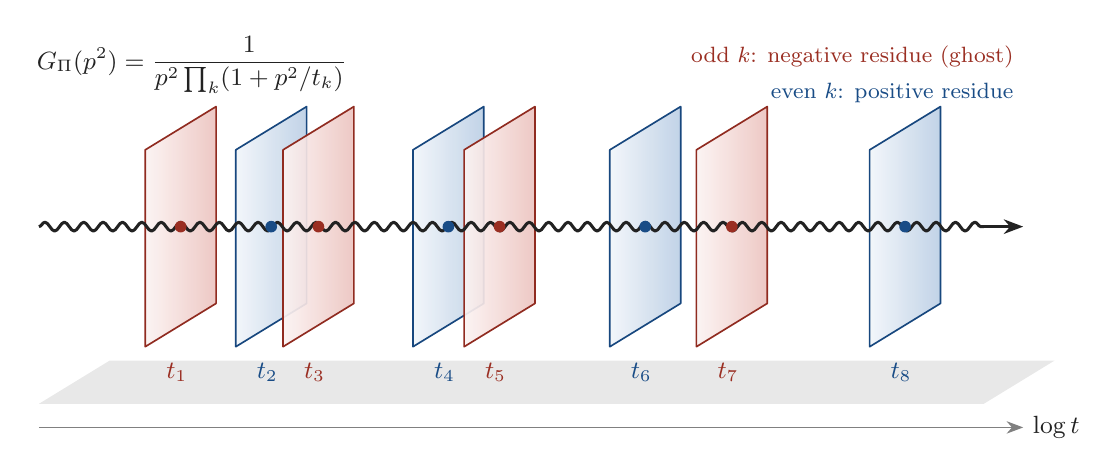
\begin{tikzpicture}[x=1cm,y=1cm,line join=round]
  % oblique depth vector
  \def\dx{0.9}\def\dy{0.55}
  \fill[gray!18] (-0.6,-2.25) -- (11.4,-2.25) -- (11.4+0.9,-2.25+0.55) -- (-0.6+0.9,-2.25+0.55) -- cycle;
  \foreach \p/\lab/\col/\h [count=\i] in {1.2/t_1/ghost/1.0, 2.35/t_2/healthy/1.0, 2.95/t_3/ghost/1.0,
      4.6/t_4/healthy/1.0, 5.25/t_5/ghost/1.0, 7.1/t_6/healthy/1.0, 8.2/t_7/ghost/1.0, 10.4/t_8/healthy/1.0} {
    \shade[left color=\col!6, right color=\col!30, opacity=0.92] (\p-\dx/2,-1.25-\dy/2) -- (\p+\dx/2,-1.25+\dy/2) -- (\p+\dx/2,1.25+\dy/2) -- (\p-\dx/2,1.25-\dy/2) -- cycle;
    \draw[\col!75!black, line width=0.6pt] (\p-\dx/2,-1.25-\dy/2) -- (\p+\dx/2,-1.25+\dy/2) -- (\p+\dx/2,1.25+\dy/2) -- (\p-\dx/2,1.25-\dy/2) -- cycle;
    \node[text=\col!80!black, font=\small] at (\p-0.05,-1.85) {$\lab$};
  }
  % graviton line through the stack
  \draw[ink, line width=1.1pt, decorate, decoration={snake, amplitude=1.6pt, segment length=7pt}]
     (-0.6,0) -- (11.4,0);
  \draw[-{Stealth[length=7pt]}, ink, line width=1.1pt] (11.35,0) -- (11.9,0);
  \foreach \p/\col in {1.2/ghost,2.35/healthy,2.95/ghost,4.6/healthy,5.25/ghost,7.1/healthy,8.2/ghost,10.4/healthy}
     \fill[\col!80!black] (\p,0) circle (2.1pt);
  % axis
  \draw[-{Stealth[length=6pt]}, gray] (-0.6,-2.55) -- (11.9,-2.55) node[right, text=ink, font=\small] {$\log t$};
  \node[font=\small, text=ink, anchor=west] at (-0.75,2.05) {$G_\Pi(p^2)=\dfrac{1}{p^2\prod_k(1+p^2/t_k)}$};
  \node[font=\footnotesize, text=ghost!80!black, anchor=east] at (11.9,2.15) {odd $k$: negative residue (ghost)};
  \node[font=\footnotesize, text=healthy!80!black, anchor=east] at (11.9,1.7) {even $k$: positive residue};
\end{tikzpicture}
\end{document}
